\documentclass[a4paper,12pt]{report}

\usepackage[utf8]{inputenc}
\usepackage{t1enc}
\usepackage[T1]{fontenc}
\usepackage[magyar]{babel}
\usepackage{indentfirst}
\usepackage{anysize}
\usepackage{graphicx}
\usepackage{sidecap}
\usepackage{subfigure}
\usepackage{amsmath, amssymb, amsfonts}
\usepackage{latexsym}
\usepackage{todonotes}
\usepackage{verbatim}

\setlength{\parindent}{0pt}
\setlength{\parskip}{1ex plus 0.5ex minus 0.2ex}
\reversemarginpar
\setlength{\marginparwidth}{2.5cm}
%\setlength{\oddsidemargin}{0cm}
%\setlength{\evensidemargin}{0cm}

\newtheorem{Tet}{Tétel}[section]
\newtheorem{Lem}[Tet]{Lemma}
\newtheorem{All}[Tet]{Állítás}
\newtheorem{Kov}[Tet]{Következmény}
\newtheorem{Def}[Tet]{Definíció}
\newtheorem{Megj}[Tet]{Megjegyzés}
\newtheorem{Jel}[Tet]{Jelölés}
\newtheorem{Pl}[Tet]{Példa}
\newtheorem{Fel}[Tet]{Feladat}
\newenvironment{Mo}{\noindent \textbf{Megoldás. }}{ $\clubsuit$}
\newenvironment{Biz}{\noindent \textbf{Bizonyítás. }}{ $\square$}

\newcommand{\noun}[1]{\textsc{#1}}
\newcommand{\todored}[1]{\todo[color=red!70, size=\footnotesize]{#1}}
\newcommand{\todoor}[1]{\todo[color=orange!90, size=\footnotesize]{#1}}

\title{Szakdolgozat}

\begin{document}


% Első két oldal:



	\thispagestyle{empty}
	\begin{center}
		{\large \noun{Eötvös Loránd Tudományegyetem \\ Természettudományi Kar} }
		\line(1,0){455}
		\vspace{80pt}
		{\Huge \noun{\textbf{Véletlen iterációk statisztikai elemzése}}}
		\vspace{20pt}
		\\BSc Szakdolgozat
		\vspace{90pt}
		\\Írta: Mészáros Ádám István\\ Matematika BSc, Matematikai elemző szakirány\\
		\vspace{35pt}
		Témavezető: Sigray István\\ Műszaki Gazdasági Tanár, Analízis tanszék\\
		\vspace{100pt}
		
\includegraphics[scale=0.21]{elte.png}
		\vspace{25pt}
		\\ 2013\\ Budapest
	\end{center}
	\tableofcontents
	\setcounter{page}{1}


%%============================================================================
%%========================== szakdolgozat tartalmi része =====================
%%============================================================================

%=======================================================
%
%				0. FEJEZET
%				KÖSZÖNETNYILVÁNÍTÁS
%
%=======================================================


	\chapter*{Köszönetnyilvánítás}
		Lorem ipsum dolor sit amet, consectetur adipisicing elit, sed do eiusmod tempor incididunt ut labore et dolore magna aliqua. Ut enim ad minim veniam, quis nostrud exercitation ullamco laboris nisi ut aliquip ex ea commodo consequat. Duis aute irure dolor in reprehenderit in voluptate velit esse cillum dolore eu fugiat nulla pariatur. Excepteur sint occaecat cupidatat non proident, sunt in culpa qui officia deserunt mollit anim id est laborum.



%=======================================================
%
%				1. FEJEZET
%				BEVEZETÉS
%
%=======================================================

	\chapter{Bevezetés}
		Lorem ipsum dolor sit amet, consectetur adipisicing elit, sed do eiusmod tempor incididunt ut labore et dolore magna aliqua. Ut enim ad minim veniam, quis nostrud exercitation ullamco laboris nisi ut aliquip ex ea commodo consequat. Duis aute irure dolor in reprehenderit in voluptate velit esse cillum dolore eu fugiat nulla pariatur. Excepteur sint occaecat cupidatat non proident, sunt in culpa qui officia deserunt mollit anim id est laborum.
	



%=======================================================
%
%				2. FEJEZET
%				A NEWTON-MÓDSZER
%
%=======================================================


	
	\chapter{A Newton-módszer}
    
    
    %=======================================================
    %
    %				2. FEJEZET
    %				A NEWTON-MÓDSZER
    %					|
    %					->	2.1 A módszer leírása
    %
    %=======================================================
        
        
		\section{A módszer leírása}
        	
			A Newton-módszer, mint a neve is mutatja, először Isaac Newton dolgozta ki, azonban a mai formáját Joseph Raphson írta le 1690-ben, ezért Newton-Raphson-módszernek is hívják. Newton a módszert eredetileg polinomokra alkalmazta, ahogy a későbbiekben majd én is teszem. A Newton-módszer egy iterációs eljárás nemlineáris egyenletek gyökeinek megtalálására, közelítésére. A módszer - valós esetben - egy geometriailag nagyon egyszerű meggondoláson alapul, amit egy kép segítségével fogok bemutatni.
			\begin{figure}[htp]
				\centering
				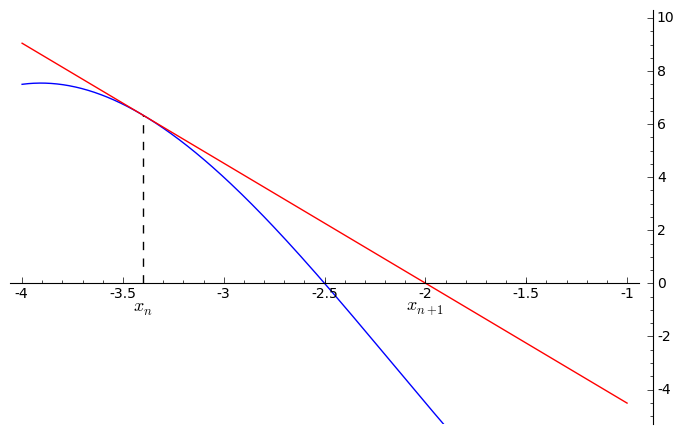
\includegraphics[scale=0.55]{kep1.png}
				\caption{Egy lépés a Newton-módszerrel}\label{k1}
			\end{figure}
			Első lépésként vegyünk egy kezdőpontot az $x$ tengelyen, amely elég közel van a gyökünkhöz. Jelöljük $x_0$-lal. Tegyük fel, hogy $n$ lépés után eljutottunk az $x_n$ pontig. Húzzunk érintőt a grafikonhoz ebben a pontban. Az érintő és az $x$ tengely metszéspontja legyen a következő pontunk, $x_{n+1}$, majd így folytassuk amíg elég közel nem kerülünk a egyenletünk gyökéhez. Tegyük fel, hogy $x_k$ közel van az $f(x)=0$ egyenlet $x^*$ gyökéhez, és $f$ kétszer folytonosan differenciálható. \todoor{Változtatás: következő mondat a Tanár úr megjegyzése alapján} Ekkor felírhatjuk $f$ elsőfokú Taylor-polinomját maradéktaggal a következőképpen
			\[ f(x^*)=f(x_k)+f'(x_k)(x^*-x_{k})+O((x^*-x_{k})^2) \]
			$f(x^*)$ lineáris közelítéséhez nincsen szükségünk az $(x^*-x_{k})^2$-es tagokra.
			\begin{eqnarray*}
				f(x^*)&\approx& f(x_k)+f'(x_k)(x^*-x_{k})\\
				0&\approx&\frac{f(x_k)}{f'(x_k)}+(x^*-x_{k})\\
				x^*&\approx & x_k-\frac{f(x_k)}{f'(x_k)}
			\end{eqnarray*}
			Definiáljunk egy lépést a közelítés jobb oldalával, így előállíthatjuk a következő iterációt
			\begin{equation}
				 \label{e2} x_{k+1}=x_k-\frac{f(x_k)}{f'(x_k)}
			\end{equation}
			\begin{Pl}
				Az alábbiakban a \ref{k1} képen ábrázolt polinommal fogok számolni.
				\[f(x)=x^3+6.5x^2+5x-12.5\]
				$f(x)=0$ egyenletnek gyöke az $x^*=-2.5$. Induljunk el az $x_0=-1$ pontból.
                \begin{center}				
                  \begin{tabular}{|r|r|r|r|}
                      \hline
                      $k$ & $x_k$     & $f(x_k)$      & $|x_k-x^*|$  \\ \hline
                      $0$ & $-1.0000$ & $-1.2000e+01$ & $1.5000e+00$ \\ 
                      $1$ & $-3.4000$ & $6.3360e+00$  & $9.0000e-01$ \\ 
                      $2$ & $-1.9982$ & $-4.5159e+00$ & $5.0177e-01$ \\ 
                      $3$ & $-2.5001$ & $8.6664e-04$  & $9.9045e-05$ \\ 
                      $4$ & $-2.5000$ & $-9.8121e-09$ & $1.1214e-09$ \\
                      \hline
                  \end{tabular}
				\end{center}
            \end{Pl}
            
    	
            
    %=======================================================
    %
    %				2. FEJEZET
    %				A NEWTON-MÓDSZER
    %					|
    %					->	2.2 Konvergencia vizsgálat
    %
    %=======================================================
        
        
		\section{Konvergencia vizsgálat}
			\begin{Jel}
            
            \todored{javaslom a k\"ovetkez\H oket a fejezet elej\'ere: Legyen $[a,b]\subset{\mathbb R}$ egy 
            intervallum, $f:[a,b]\to {\mathbb R}$ k'etszer folytonosan differenci'lhat\'o. E fejezet sor\'an azt viysg\'aljuk, hogy milyen esetben tudjuk garant\'alni azt, hogy a Newton iter\'aci\'o $f$ egy gz\"ok\'ehez konverg\'al.
            
            (Ezek ut\'an a fejezet t\'eteleibe) e felt\'etelt nem kell be\'\i rni, ugyanis hol szerepeltek, hol nem.}
				\todoor{Változtatás: A jelölés részt előrrébb hoztam, hogy a tételt precízebben ki tudjam mondani, és $m_1$, $M_2$ definícióit a Tanár úr megjegyzése alapján átírtam.}$m_1:=\smash{\displaystyle \min_{x \in [x_k,x^*]}} |f'(x)|$, $M_2:=\smash{\displaystyle \max_{x\in [x_k,x^*]}} |f''(x)|$, $C:=\frac{M_2}{2m_1}$
			\end{Jel}
			\begin{Tet}
			\label{t2} Tegyük fel, hogy $f\in C^2[a,b]$, és egyértelműen létezik $x^*\in [a,b]$ amelyre $f(x^*)=0$, továbbá $m_1>0$. \todoor{Változás: töröltem $M_2$-s feltételt}Ekkor, ha a Newton-módszer konvergens, akkor másodrendben konvergál a gyökhöz.
			\end{Tet}
			\begin{Biz}
				Írjuk fel $f$ $x_k$ körüli másodfokú Taylor-polinomját Lagrange maradéktaggal az $x^*$ pontban 
				\begin{eqnarray}
					f(x^*)&=&f(x_k)+f'(x_k)(x^*-x_{k})+\frac{f''(\xi)}{2}(x^*-x_{k})^2 \\
					0&=&\frac{f(x_k)}{f'(x_k)}+(x^*-x_{k})+\frac{\frac{f''(\xi)}{2}(x^*-x_{k})^2}{f'(x_k)}\\
					\label{e1} x^*&=&x_k-\frac{f(x_k)}{f'(x_k)}-\frac{f''(\xi)}{2f'(x_k)}(x^*-x_{k})^2
				\end{eqnarray}
				Ahol $\xi \in (x_k,x^*)$. Vonjuk ki a \ref{e2} egyenletből a \ref{e1}-t
				\begin{eqnarray*}
					x_{k+1}-x^*&=&\left(x_k-\frac{f(x_k)}{f'(x_k)}\right) - \left(x_k-\frac{f(x_k)}{f'(x_k)}-\frac{f''(\xi)}{2f'(x_k)}(x^*-x_{k})^2\right)\\
					x_{k+1}-x^*&=&\frac{f''(\xi)}{2f'(x_k)}(x^*-x_{k})^2\leq C |x^*-x_k|^2
				\end{eqnarray*}
				Vagyis a következőt kapjuk
				\begin{equation}
					\label{e3}|x_{k+1}-x^*|\leq C |x^*-x_k|^2
				\end{equation}
				Vagyis hogyha a Newton-módszer konvergens, akkor másodrendben konvergál.
			\end{Biz}
			
    A másodrendű konvergencia azt jelenti, hogy a hiba legalább négyzetesen csökken, vagyis a helyes jegyek száma nagyjából megduplázódik a lépésenként.
            
			Hogyan tudjuk garantálni a konvergenciát? \todoor{Változtatás: Tanár úr megjegyzése alapján a következő mondat} \ref{e3} egyenlőtlenséget a következőképpen tudjuk iterálni $x^*$ közelében
			\begin{eqnarray}
				|x_k-x^*|&\leq& C |x^*-x_{k-1}|^2\\
				&\leq & C\left |C|x^*-x_{k-2}|^2\right |^2=C^3|x^*-x_{k-2}|^4\\
				&\leq & \ldots\leq C^{2^k-1} |x^*-x_0|^{2^k}\label{e4}			
			\end{eqnarray}
			Vagyis $|x_k-x^*|\leq C^{2^k-1}|x^*-x_0|^{2^k}$. Szeretnénk, ha a következő teljesülne
			\[ \lim_{k \to \infty} |x^*-x_k|=0\]
			Ha a \ref{e4}-as egyenletben az egyenlőtlenség jobb oldala tart nullához, akkor a Rendőr-elv alapján ez teljesül.
			\[ C^{2^k-1}|x^*-x_0|^{2^k}=q^{2^k-1}|x^*-x_0| \] 
			Ez akkor és csak akkor tart nullához, ha $q<1$.
			\[q=C|x^*-x_0|=  \frac{M_2}{2 m_1} \left |x^*-x_0 \right | < 1 \]
			Átrendezve
			\[ |x_0-x^*|<  \frac{2 m_1}{M_2} \]
			Ezek alapján a következő tételt mondhatjuk ki
			\todoor{Változtatás: beleírtam, hogy van egy $I$ intervallumunk, és $m_1$, $M_2$ definícióját átírtam erre az intervallumra. Úgy gondolom így áthidaltam azt a problémát, hogy eddig ezek a konstansok függtek $x_k$-tól. A 3. pontot átírtam $M_2$ jelölés felhasználásával.}
            \begin{Tet}
				Legyen $I$ egy adott intervallum, és $m_1:=\smash{\displaystyle \min_{x \in I}} |f'(x)|$, $M_2:=\smash{\displaystyle \max_{x\in I}} |f''(x)|$. Tegyük fel a következőket	
				\begin{enumerate}
					\item $f(x)$-hez $!\exists x^*\in I$, amire $f(x^*)=0$
					\item $f(x)$ kétszer folytonosan deriválható az $I$ intervallumon
					\item $M_2<\infty$
					\item $\forall x \in I$-re $f'(x) \neq 0$ 
					\item $x_0 \in \left (x^*-\frac{2 m_1}{M_2},x^*+\frac{2 m_1}{M_2}\right )$	
				\end{enumerate}
				Ekkor $\smash{\displaystyle \lim_{k\to \infty} }x_k= x^*$.
			\end{Tet}
            \todoor{Változtatás: A következő eddig megjegyzés környezetben volt}
			Ezeket sajnos elég nehéz garantálni. Például az 5. feltételhez tudnunk kell, hogy mi a gyök, aminek a meghatározására alkalmaznánk a módszert. A 4. feltétel ellenőrzése szintén bonyolult, hiszen ehhez először meg kellene határoznunk a derivált gyökeit, amivel szintén az eredeti problémához jutunk.
            \begin{Tet}
				\label{t1}
				Tegyük fel, hogy $f\in C^2[a,b]$, és egyértelműen létezik $x^*\in [a,b]$ amelyre $f(x^*)=0$, továbbá $x_0\in [a,b]$, $\forall x \in (x^*,x_0)$-re $f'(x)$,$f''(x) \neq 0$, és $x_0$-ra teljesül, hogy $f(x_0)f''(x_0)>0$, akkor $x_k$ szigorúan monoton tart a gyökhöz.
			\end{Tet}
            \todoor{Változtatás: A tétel feltételeit átírtam hasonló stílusúra mint amiket előzőekben már használtam}
			\begin{Biz}
				Négy esetünk van.
				\begin{enumerate}
					\item $x_0>x^*$, $f(x_0)>0$
					\item $x_0>x^*$, $f(x_0)<0$
					\item $x_0<x^*$, $f(x_0)>0$
					\item $x_0<x^*$, $f(x_0)<0$
				\end{enumerate}	
				Az esetek bizonyítása nagyban hasonlít, ezért csak az elsőt látjuk be. Mivel $f(x_0)>0$ és $f(x_0)f''(x_0)>0$, ezért $f''(x_0)>0$. Továbbá $(x^*,x_0)$-n $f'(x)\neq 0$, ezért az vagy mindenhol pozitív, vagy mindenhol negatív. 
				\begin{eqnarray}
					\label{e6}0&<&f(x_0)\\
					\label{e7}&=&f(x_0)-f(x^*)\\
					\label{e8}&=&f'(\xi)\underbrace{(x_0-x^*)}_{>0}
				\end{eqnarray}
				\ref{e7} $\Rightarrow$ \ref{e8} a Lagrange-féle középérték tétel miatt, valamilyen $\xi \in (x^*,x_0)$-re. Ez azt jelenti, hogy $f'(\xi)>0$, amiből következik, hogy $\forall x\in (x^*,x_0): f'(x)>0$. Ez alapján a következőt tudjuk
				\begin{eqnarray*}
					x_{k+1}&=&x_k-\underbrace{\frac{f(x_k)}{f'(x_k)}}_{>0} \\
					x_{k+1}&<&x_k
				\end{eqnarray*}
				Vagyis az $x_k$ sorozat szigorúan monoton csökkenő. Használjuk ismét a Lagrange-féle középérték tételt
				\[0<f(x_k)=f(x_k)-f(x^*)=\underbrace{f'(\xi)}_{>0}(x_k-x^*)\]
				Tehát $x_k>x^*$ azaz $x_k$ sorozat korlátos. A korlátosságból, és a monotonitásból következik, hogy $x_k$ konvergens. Tegyük fel, hogy $x_k\to \tilde{x}^*$.
				\begin{eqnarray*}
					\lim_{k \to \infty} x_{k+1} &=& \lim_{k \to \infty} x_k - \dfrac{\lim\limits_{k \to \infty} f(x_k)}{\lim\limits_{k \to \infty} f'(x_k)}\\
					\tilde{x}^*&=&\tilde{x}^*-\dfrac{f(\tilde{x}^*)}{f'(\tilde{x}^*)}\\
					\dfrac{f(\tilde{x}^*)}{f'(\tilde{x}^*)}&=&0
				\end{eqnarray*}
				Ez csak akkor lehetséges, ha $f(\tilde{x}^*)=0$, viszont $x^*$ gyök egyértelmű, ezért $x^*=\tilde{x}^*$.
			\end{Biz}
            
            
    %=======================================================
    %
    %				2. FEJEZET
    %				A NEWTON-MÓDSZER
    %					|
    %					->	2.3 Leállási feltétel
    %
    %=======================================================
            
        \todoor{Megjegyzés: Ebben a részben nem vagyok biztos, \cite[p. 145]{na}-ben találtam az 5.2.3. tétel, de nem a Newton-módszerre szól hanem általánosan a fixpont iterációkra, de átírtam egy-két dolog, ahogy szerintem specifikus a Newton-módszerre.}    
		\section{Leállási feltétel}
			\begin{Jel}
				$m_1:=\smash{\displaystyle \min_{x \in (a,b)} } \left| \left( \dfrac{f(x)}{f'(x)} \right)' \right|$
			\end{Jel}
			\begin{Tet}
				Tegyük fel, hogy $f\in C^2[a,b]$ és $m_1>0$. Ekkor ha valamilyen $\varepsilon >0 $-ra és k indexre
				\begin{equation}
					\label{e5} \left| \frac{x_{k+1}-x_k}{x_k} \right |\leq \frac{\varepsilon}{\varepsilon+1}m_1
				\end{equation}
				akkor $|x_k-x^*|\leq \varepsilon|x^*|$.
			\end{Tet}
			\begin{Biz}
				Rendezzük át a \ref{e2} egyenletet és alkalmazzuk a Lagrange-féle középérték tételt.
				\begin{eqnarray*}
					| x_{k+1} - x_{k}|&=& \left| \frac{f(x_k)}{f'(x_k)} \right| \\
					&=& \left| \frac{f(x_k)}{f'(x_k)}- \frac{f(x^*)}{f'(x^*)} \right| \\
					&=&\left| \left(\frac{f(\xi)}{f'(\xi)}\right)'\right| \cdot |x_k-x^*|
				\end{eqnarray*}			
				ahol $\xi \in (x*,x_k)$
				\[| x_{k+1} - x_{k}|\geq m_1 |x_k-x^*| \]
				Fejezzük ki \ref{e5} -t $m_1$-re és helyettesítsük be.
				\begin{eqnarray*}
					| x_{k+1} - x_{k}|&\geq& \frac{|x_{k+1}-x_k|}{|x_k|}\cdot \frac{\varepsilon+1}{\varepsilon}\cdot |x_k-x^*|\\
					\varepsilon |x_k|&\geq& \varepsilon  |x_k-x^*| + |x_k-x^*|\\
					 |x_k-x^*|&\leq &\varepsilon (|x_k|- |x_k-x^*|)\\
					&\leq& \varepsilon(|x_k-x_k+x^*|)=\varepsilon |x^*|
				\end{eqnarray*}
			\end{Biz}
			\begin{Kov}
				Tegyük fel, hogy szeretnénk $e$-nél kisebb hibával közelíteni $x^*$-ot. Mivel $|x^*|\leq\max \{ |a|,|b| \}$, ha ismerünk, egy olyan $\varepsilon$ számot, amelyre teljesül a tételbeli feltétel, és $\varepsilon \max \{|a|,|b|\} \leq e$, akkor
				\[ |x_k-x^*|\leq \varepsilon |x^*| \leq \varepsilon \max \{|a|,|b|\} \leq e \]
			\end{Kov}
			\todoor{Változtatás: Innentől kezdve minden új}
			Sajnos ez a leállási feltétel nem túl hasznos, hiszen minden lépésnél újabb $\varepsilon$-t kell keresnünk, ami műveletigényes.


    %=======================================================
    %
    %				2. FEJEZET
    %				A NEWTON-MÓDSZER
    %					|
    %					->	2.4 Komplex eset
    %
    %=======================================================


		\section{Komplex eset}
             Érdemes megvizsgálni a módszert komplex gyökkel rendelkező egyenletekre is. Ekkor a fentiekkel analóg állítások mondhatók ki. A komplex eset geometriai meggondolása is hasonló. Feleltessük meg a $z=x+yi \in \mathbb{C}$ számokat $(x,y)\in\mathbb{R}^2$ vektorokkal. Legyen $f(z)=u+vi=u(x,y)+v(x,y)i$ analitikus függvény. $|f(z)|=\sqrt{u^2(x,y)+v^2(x,y)}$. $z_k=x_k+y_ki$ ahol $f$, és $f'$ sem 0. Legyen $T_k$ $|f(z)|$ érintő síkja a $(x_k,y_k)$ helyen, és legyen $L_k$ az $xy$ sík és $T_k$ metszésvonala. Belátható, hogy ekkor \[z_{k+1}=x_{k+1}+y_{k+1}i=z_k-\frac{f(z_k)}{f'(z_k)}\] megfelel annak az $(x_{k+1},y_{k+1})$ pontnak amelyik az $L_k$ egyenesen legközelebb van $(x_k,y_k)$ ponthoz. (\ref{k6}) \cite[p. 809]{Yau98}. A lépés iránya ezáltal ellentétes $|f(z)|$ gradiensével a $z_k$ pontban.
            \begin{figure}[htp]
				\begin{center}
				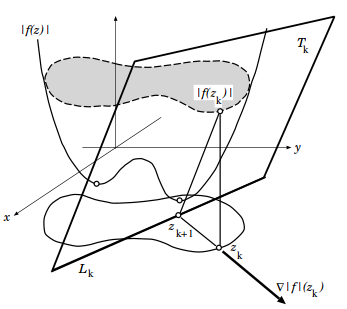
\includegraphics[scale=0.7]{kep6.png}
				\caption{A komplex eset geometriai meggondolása \cite[p. 807]{Yau98}} \label{k6}
				\end{center}
			\end{figure}
			Meggondolható, hogy ez valós esetben ugyanazt jelenti mint eddig, hiszen a két sík metszésvonala helyett, az $x$ tengely és $|f(x)|$ érintő egyenesének metszéspontját vesszük, ami megegyezik az $x$ tengely és $f(x)$ érintőjének metszéspontjával.	 	

            Vegyük például a $f(x)=x^2-2i$ komplex együtthatós polinomot, amelynek az $1+i$ és a $-1-i$ a gyökei. $|f|$ gradiensénél (\ref{k7} ábra) valamivel jobb szemléltetés végett definiáljuk a következő vektormezőt
			\[g(x,y)=\left(\mathrm{Re} \left\{ -\frac{f(x+yi)}{f'(x+yi)} \right \} ,\mathrm{Im} \left\{-\frac{f(x+yi)}{f'(x+yi)}\right \} \right)\]
            Ezt ábrázolva láthatjuk, hogy az esetünkben hogyan fog haladni a komplex síkon a módszer. A \ref{k4} ábrákon jelöltem $1-0.5i$-ből indított módszer pontjait is. A kezdőpont pirossal van ábrázolva, ami az iterációs lépésekkel átvált sárgába.
			\begin{figure}[htp!]
           		\subfigure[$-\nabla|f(z)|$ és négy iterációs lépés az $1-0.5i$-ből]{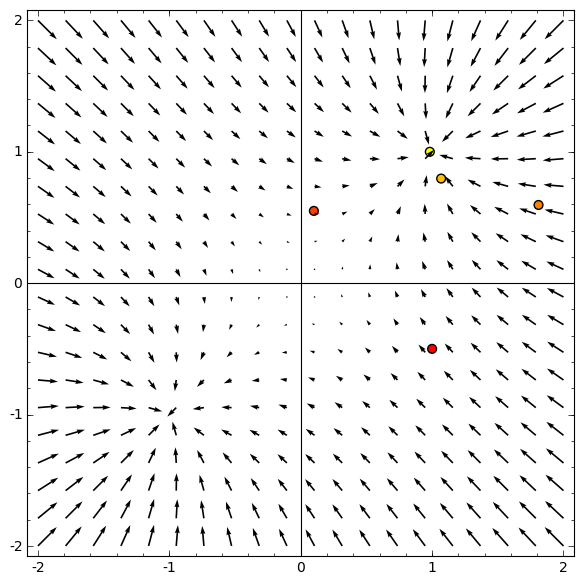
\includegraphics[scale=0.5]{kep7.png} \label{k7}}
                \hfill
            	\subfigure[$g(x,y)$ és négy iterációs lépés az $1-0.5i$-ből]{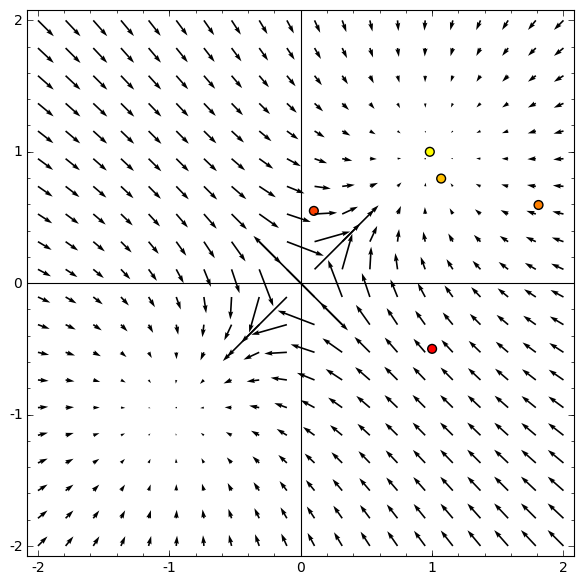
\includegraphics[scale=0.5]{kep4.png}}
           	 	\caption{A lépés irányán túl a (b) ábra a lépés nagyságát is szemlélteti} \label{k4}
           	\end{figure}
            \begin{Pl}
				\ref{k4} ábra számokkal, vagyis $f(x)=x^2-2i$ gyökét keressük $1-0.5i$ kezdőponttal.
				\begin{center}				
                    \begin{tabular}{|r|r|r|r|}
                        \hline
                        $k$ & $z_k$                & $|f(z_k)|$    & $|z_k-z^*|$  \\ \hline
                        $0$ & $1.00000 - 0.50000i$ & $3.0923e+00$  & $1.5000e+00$ \\ 
                        $1$ & $0.10000 + 0.55000i$ & $ 1.9125e+00$ & $1.0062e+00$ \\ 
                        $2$ & $1.81000 + 0.59500i$ & $2.9261e+00$  & $9.0561e-01$ \\ 
                        $3$ & $1.06891 + 0.79611i$ & $5.8966e-01$  & $2.1522e-01$ \\ 
                        $4$ & $0.98262 + 0.99980i$ & $4.8935e-02$  & $1.7377e-02$ \\ 
                        $5$ & $1.00008 + 0.99992i$ & $3.0464e-04$  & $1.0771e-04$ \\ 
                        $6$ & $1.00000 + 1.00000i$ & $1.1601e-08$  & $4.1015e-09$ \\
                        \hline
                    \end{tabular}
				\end{center}
            \end{Pl}
			Láthatjuk, a módszer nem csak komplex gyökökkel rendelkező valós polinomokra működik, de komplex együtthatós polinomokra is. Azonban ha egy valós polinom komplex gyökét szeretnénk meghatározni, akkor szükséges, hogy a kezdőpontunk képzetes része eltérjen nullától, különben az iterációs lépés tulajdonásága miatt $\forall z_k\in \mathbb{R}$ (\ref{k5} ábra).
            
            \begin{figure}[htp]
				\begin{center}
				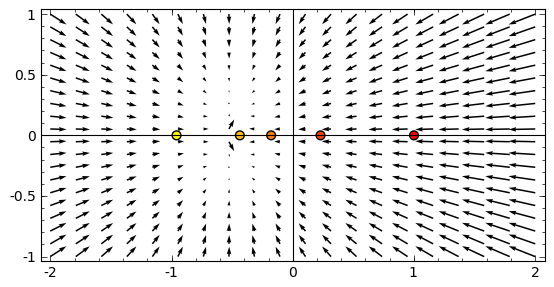
\includegraphics[scale=0.62]{kep5.png}
				\caption{$x^2 + x + 0.3125$ komplex gyökeinek keresése valós kezdőpontból} \label{k5}
				\end{center}
			\end{figure}

			\todoor{Változás: (2013.04.13) Innentől a fejezet végéig új} 
            A komplex síkon minden gyökhöz tartozik egy vonzáskörzet, amely halmazból az iterációt indítva az adott gyökhöz konvergál a módszer. A teljes komplex síkhoz, ezenkívül hozzátartoznak azon ponthalmazok ahonnan a módszer nem konvergens. Számos komplex függvényre ezen halmazok határai egy fraktált határoznak meg. (\ref{k10} ábra)
			
			\begin{figure}[htp]
				\begin{center}
				{%
					\setlength{\fboxsep}{0pt}%
					\setlength{\fboxrule}{1pt}%
					\fbox{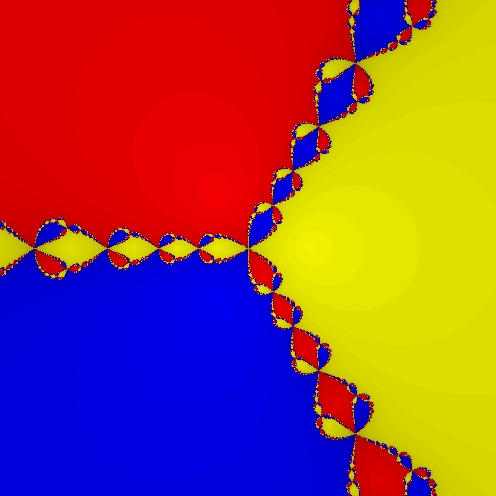
\includegraphics[scale=0.35]{fractal.png}}
				}%
				\caption{$x^3-1$ komplex gyökeihez tartozó halmazok a $\{a+bi:a,b\in[-5,5]\}$ síkrészen. A piros részből indított iteráció $-1/2+i\sqrt{3}/2$-höz konvergál, a kék részről ennek komplex konjugáltjához, és a sárga részről $1$-hez.} \label{k10}
				\end{center}
			\end{figure}
			
			Érdekes kérdés, hogy meg tudjuk-e határozni a gyökökhöz tartozó vonzáskörzeteket adott függvényekre. A másodfokú polinomokra a következő tételt tudjuk
			\begin{Tet}[Arthur Cayley, 1897]
				Legyen $p$ komplex másodfokú polinom, melynek $\alpha$ és $\beta$ két különböző gyöke. Legyen $L$ az $\alpha$-t és $\beta$-t összekötő szakasz függőleges felezővonala. Ekkor, ha a Newton-módszert alkalmazzuk $p$-re, a gyökökhöz tartozó $B(\alpha)$ és $B(\beta)$ vonzáskörzetek, az $L$ egyenes által szétválasztott komplex félsíkok.
			\end{Tet}


%=======================================================
%
%				3. FEJEZET
%				MÓDOSÍTOTT MÓDSZER POLINOMOKRA
%
%=======================================================
    
    
    
	\chapter{Módosított módszer polinomokra}
		Adott a Newton-módszer, amit az előző fejezetben vizsgáltunk. Tudjuk, hogyha az $x_k$ sorozat konvergens, akkor másodrendben konvergál a gyökhöz (\ref{t2}), sőt bizonyos feltételeket biztosítva monoton konvergenciát tudtunk biztosítani (\ref{t1}). Azonban sok esetben a módszer nem konvergens. Szeretnénk egy olyan módszert, amely viszonylag gyorsan és sok helyről konvergens.
        \todored{A sz\"ovegbe menjen: A probl\'ema ugyanis az, hogy a konvergenciavizsg\'alataink csak lok\'alisak voltak, azaz csak akkor garant\'alt\'ak a konvergenci\'at, amikor a gy\"okh\"oz kell\H oen k\"ozelr\H ol indultunk. Ez term\'eszetesen nem teljes\"ul egy v\'eletlen\"ul v\'alasztott  kezd\H opont eset\'en. Ilyen esetben csak abban lehet rem\'enykedni, hogy az iter\'aci\'o "v\'eletlens\'egb\H ol" egyik l\'ep\'es sor\'an k\"ozel ker\"ul a gy\"okh\"oz. 
        
Ennek a k\'erd\'esnek nagy elm\'elete van, \'es paradox m\'odon a komplex esetben lehet t\"obbet tudni, mint a val\'os esetben.}
  
      
      
    %=======================================================
    %
    %				3. FEJEZET
    %				MÓDOSÍTOTT MÓDSZER POLINOMOKRA
    %					|
    %					->	3.1 Motiváció
    %
    %=======================================================
      
      
      
		\section{Motiváció}
						Vizsgáljuk meg, hogy egy polinom hogyan viselkedik a \ref{t1} tétel alapján, vagyis honnan indulva garantált a monoton konvergencia.
			\begin{figure}[htp]
				\centering
				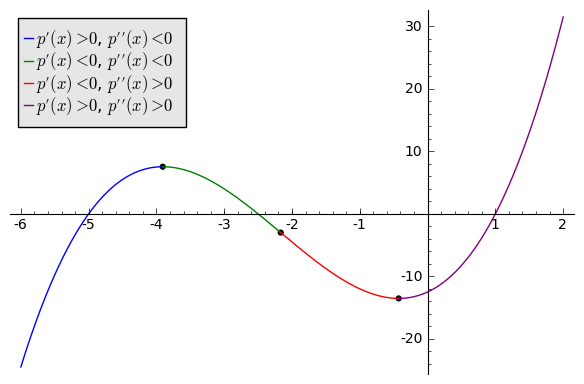
\includegraphics[scale=0.6]{kep2.png}
				\caption{Egy polinom felosztása az első és második deriváltjának viselkedése alapján}\label{k2}
			\end{figure}
			A tétel feltételei alapján a kezdőpontunk és a gyök közötti intervallumon sem a függvény deriváltja, sem a második deriváltja nem lehet nulla. Ez négy lehetőséget ad melyet a \ref{k2} ábrán szemléltettem. Mint az ábrán is látható előfordulhat olyan eset, amikor egy ilyen intervallumon nincsen gyöke a polinomnak. Azonban amelyik intervallumon van, ott vagy a gyök előtti, vagy utáni részről véve a kezdőpontunkat a feltételek teljesülnek.
			\begin{figure}[htp]
				\centering
				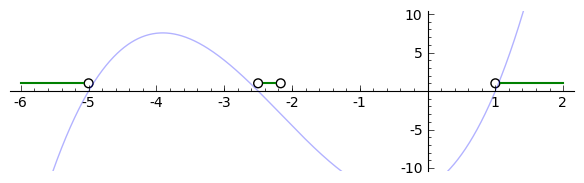
\includegraphics[scale=0.6]{kep3.png}
				\caption{Megfelelő intervallumok a kezdőpont választáshoz \ref{t1} tétel alapján}\label{k3}
			\end{figure}
			Láthatjuk, hogy esetünkben a kezdőpontunknak alkalmas intervallum majdnem lefedi a számegyenest, de pont a gyökök közelében kimaradnak kisebb részek, és bár monoton és másodrendű konvergencia garantált például a két szélső intervallumban, ha távolról indulunk, előfordulhat hogy lassú lesz a módszer.
			
			Ha egy polinomot leosztunk egy másik polinommal, és a két polinomnak nem egyezik meg valamelyik gyöke, akkor egy olyan függvényt kapunk amelynek a gyökei megegyeznek az eredeti polinomunkéval. Ugyanis legyen $p_1(x)$ a polinomunk amelyiknek a gyökeit keressük, és osszuk le $p_2(x)$ polinommal. Legyen $x^*$ gyöke $p_1(x)$-nek. Ekkor
			\[ \frac{p_1(x^*)}{p_2(x^*)}=\frac{0}{p_2(x^*)}=0\]
			
			Felvetődik tehát az ötlet, hogy hajtsuk végre a Newton-módszert a $\frac{p_1(x)}{p_2(x)}$ egyenlet gyökeinek keresésére. Vegyük azt a speciális esetet amikor $p_2(x)=p_1'(x)$. Ha $p_1(x)$-nek nincs többszörös gyöke, akkor a módosított egyenletünknek ugyanazok a gyökei.
			\begin{figure}[htp]
           		\subfigure[Egy polinom és a módosított egyenlete]{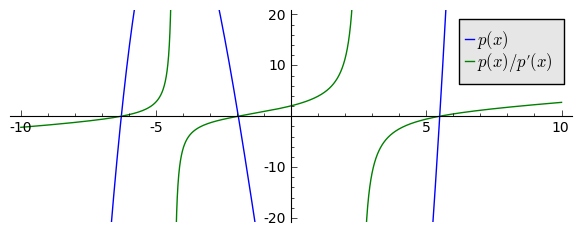
\includegraphics[scale=0.5]{sage8.png} \label{k8}}
           		\hfill
            	\subfigure[Megfelelő intervallumok a kezdőpont választáshoz \ref{t1} tétel alapján]{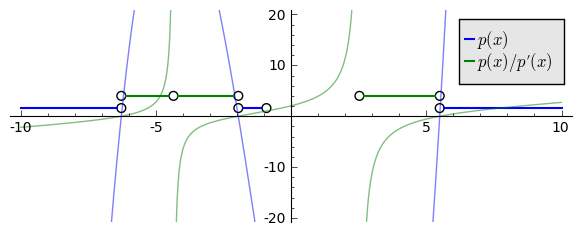
\includegraphics[scale=0.5]{sage9.png} \label{k9}}
                \caption{}
           	\end{figure}
            
    

    %=======================================================
    %
    %				3. FEJEZET
    %				MÓDOSÍTOTT MÓDSZER POLINOMOKRA
    %					|
    %					->	3.2 A módszer
    %
    %=======================================================
        
            
            \section{A módszer}
            
            Ahogyan a \ref{k9} ábrán látható a két egyenlet konvergenciát garantáló intervallumai jól kiegészítik egymást. Ez alapján az az ötletünk támadhat, hogyha véletlenszerűen váltogatjuk az egyenletet amire a módszert alkalmazzuk, jó eséllyel eljutunk az egyenletünk valamelyik gyökéhez.
			
			Tehát adott $p$ polinom amelynek a gyökeit keressük. Ekkor vegyük azt az iterációt aminek egy lépését $0.5$ valószínűséggel a (\ref{e9}) iterációval tesszük, és $0.5$ valószínűséggel (\ref{e10}) iterációval. 
			
			\begin{eqnarray}
				\label{e9}x_{k+1}&=&x_k- \frac{p(x_k)}{p'(x_k)}\\
				\label{e10}x_{k+1}&=&x_k-\frac{\frac{p(x_k)}{p'(x_k)}}{\left(\frac{p(x_k)}{p'(x_k)}\right)'}=x_k-\frac{p(x_k)p'(x_k)}{p'(x_k)^2-p''(x_k)p(x_k)}
			\end{eqnarray}
			
            \begin{Pl} Az alábbiakban egy olyan harmadfokú polinomon végzem el az iterációt aminek az együtthatóit $-50$ és $50$ között véletlenszerűen generáltam.
            	\[f(x)=-49.6776x^3+36.1231x^2-1.1662x-20.4780\]
                \begin{center}
                \begin{tabular}{|r|r|r|r|r|}
               		\hline
                	$k$ & lépés     & $x_k$                 & $|f(x_k)|$   & $|x_k-x^*|$  \\ \hline
                	$0$ & -         & $1+i$                 & $8.2695e+01$ & $5.5794e-01$ \\ 
                	$1$ & \ref{e9}  & $0.78752 + 0.72275i$  & $2.0696e+01$ & $2.0946e-01$ \\ 
                	$2$ & \ref{e10} & $0.60295 + 0.54236i$  & $3.4869e+00$ & $4.9152e-02$ \\ 
                	$3$ & \ref{e9}  & $0.64583 + 0.57250i$  & $2.7337e-01$ & $3.6089e-03$ \\ 
                	$4$ & \ref{e10} & $0.64227 + 0.57184i $ & $1.3524e-03$ & $1.7911e-05$ \\ 
                	$5$ & \ref{e9}  & $0.64228 + 0.57183i$  & $3.3361e-08$ & $4.4183e-10$ \\
                	\hline
                \end{tabular}
                \end{center}
                
            \end{Pl}
            
            \begin{Pl}
            	Egy szemléletesebb példaként hajtsuk végre a módszert a következő polinomon: $x_0=5$ kezdőponttal \[p(x)=x^3+2x^2-5x-6\]
            \begin{figure}[htp!]
           		\centering
                \subfigure[Az első lépést $p$-n végezzük: $x_1=3.4$]{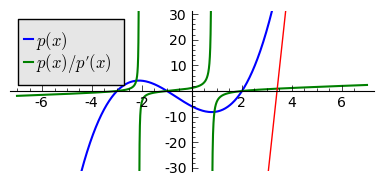
\includegraphics[scale=0.71]{0.png}}
                \hspace{3mm} % két kép közötti távolság
               	\subfigure[A második lépést is $p$-n végezzük: $x_2=2.4891$]{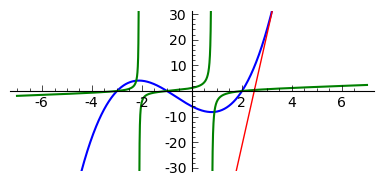
\includegraphics[scale=0.71]{1.png}}\\
                \subfigure[A harmadik lépést $p/p'$-n végezzük: $x_3=1.9040$]{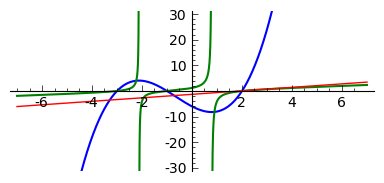
\includegraphics[scale=0.71]{2.png}}
                \hspace{3mm} % két kép közötti távolság
               	\subfigure[A negyedik lépést $p$-n végezzük: $x_4=2.0053$]{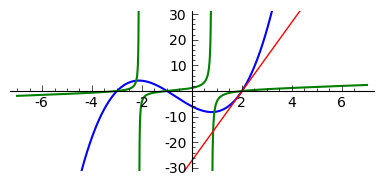
\includegraphics[scale=0.71]{3.png}}
           	 \end{figure}
             
             Látszódik az ábrákon, hogy a negyedik lépéssel elég közel kerültünk a gyökhöz, az ábrákat továbbfolytatni ezáltal fölösleges helyfoglalás lenne, viszont a következő lépés megtalálja az $x^*=2$ gyököt.
            \end{Pl}
    %=======================================================
    %
    %				3. FEJEZET
    %				MÓDOSÍTOTT MÓDSZER POLINOMOKRA
    %					|
    %					->	3.3 Elemzés
    %
    %=======================================================
				
			\section{Elemzés}
				A dolgozat következő szakaszában az imént bevezetett módszert fogjuk több szempontból megvizsgálni. A vizsgálathoz több helyen a GNU Octave programnyelvet használom, ami szinte teljesen kompatibilis a MATLAB-bal, emellett ingyenes.
				
				Egy iterációs eljárás vizsgálásakor elsősorban az érdekelhet minket, hogy konvergens-e a módszer, és ha igen akkor milyen gyorsan konvergál. 
				
				




% irodalomjegyzék
	\begin{thebibliography}{99}
    	\bibitem{jr} E. T. Whittaker, G. Robinson, ``The Newton-Raphson Method'' \emph{The Calculus of Observations: A Treatise on Numerical Mathematics, 4th ed.}, New York: Dover, pp. 84-87, 1967. 
		\bibitem{aa} Faragó István, \emph{Alkalmazott analízis 1}, előadás jegyzet 2012.
        \bibitem{na} Faragó István, Horváth Róbert, ``Nemlineáris egyenletek és egyenletrendszerek megoldása'' \emph{Numerikus módszerek}, Typotex 2011.
        \bibitem{Yau98} Lily Yau, Adi Ben-Israel ``The Newton and Halley Methods for Complex Roots'', \emph{The American Mathematical Monthly} Vol. 105, No. 9, November 1998. % http://folk.uib.no/ssu029/Pdf_file/Yau98.pdf
		\bibitem{calculus} P.D. Straffin, C.C.T. Benson, \emph{Calculus Problems for a New Century}, Mathematical Association of America 1993.

        
	\end{thebibliography}
\end{document}